\section{Clipping}

\textit{Objekte ausserhalb des Viewingbereichs nicht darstellen}

\begin{itemize}
    \item Vermeiden von unnötiger Rasterisierung
    \item Ressourcen schonen
\end{itemize}

\subsection{Verfahren}
\begin{itemize}
    \item Scissering \\
    alle Pixel berechnen \& darstellen wenn im Fenster

    \item Temporärer Buffer \\
    zeichnen in einem temporären Buffer, welcher dann Kopiert wird

    \item Analytische Berechnung derjenigen Teile, die im Innern des Fensters liegen

\end{itemize}

\subsection{Clipping von Linien}

\textit{Brute Force Algorithmus: Alle Schnittpunkte berechnen, falls mind. ein Endpunkte ausserhalb Kappungsrechteck}

\subsubsection{Clipping von Linien nach Cohen-Sutherland}


\begin{enumerate}
    \item Die ganze Ebene wird in Bereiche unterteilt
    \item Durch Vergleichen der Bereiche in denen die Endpunkte liegen, wird entschieden ob die Linie einfach akzeptiert oder abgelehnt werden kann
    \item Ist dies nicht der Fall, wird die Linie in zwei Teile geteilt, wovon eines abgelehnt wird, mit dem anderen wird zu Schritt 2 zurückgekehrt
\end{enumerate}

\begin{tabular}{cl}
    \multirow{3}{*}{
        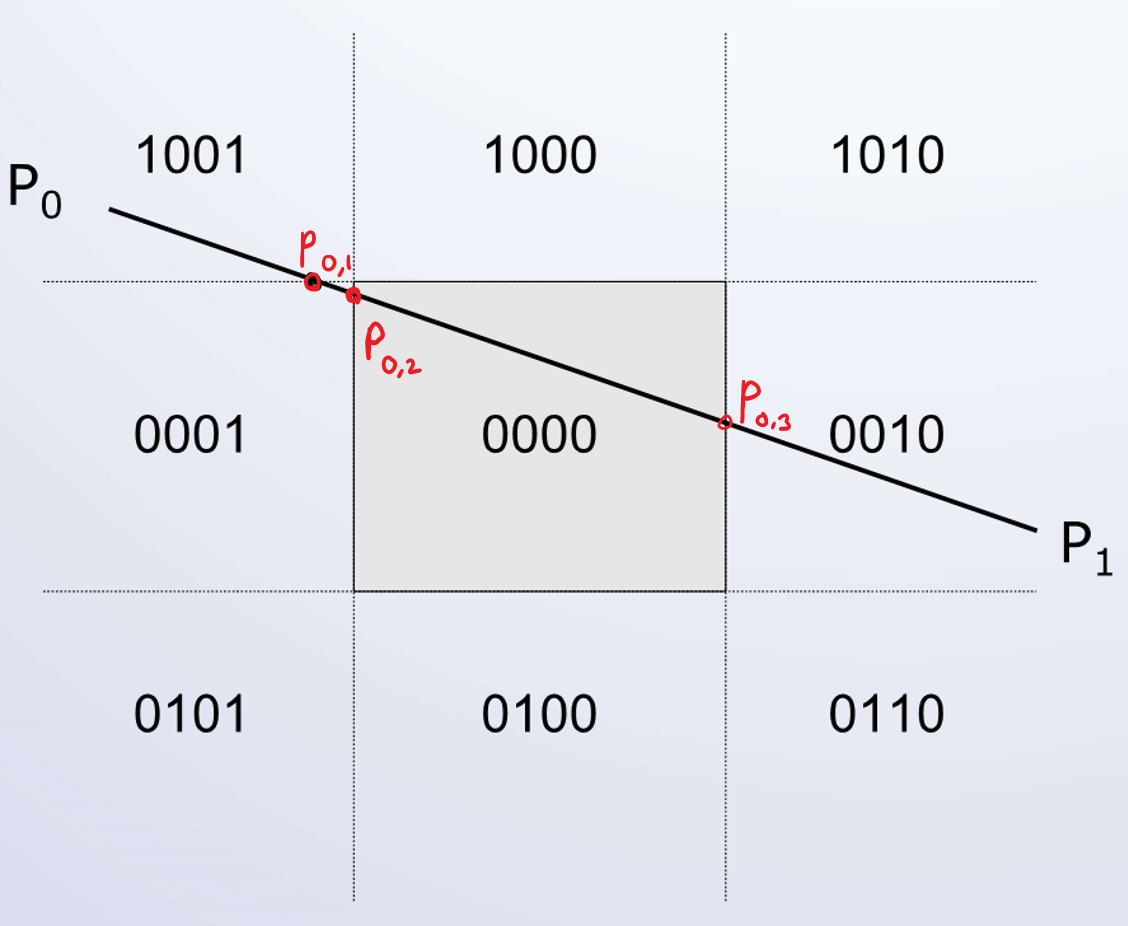
\includegraphics[width=0.3\textwidth]{assets/clipping_Cohen-Sutherland.png}
    } & \begin{tabular}{rl}
            code($P_0$) & $1001$ \\
            code($P_1$) & $0010$ \\
            \hline
            AND & $0000$ \\
        \end{tabular}
     \\
    & \begin{tabular}{rl}
        code($P_{0,2}$) & $0000$ \\
        code($P_1$) & $0010$ \\
        \hline
        AND & $0000$ \\
    \end{tabular} \\
    & \begin{tabular}{rl}
        code($P_{0,3}$) & $0000$ \\
        code($P_1$) & $0010$ \\
        \hline
        \& & $0000$ \\
    \end{tabular} \\
    & Resultat Linie: \\
    & \begin{tabular}{rl}
        code($P_{0,2}$) & $0000$ \\
        code($P_{0,3}$) & $0000$ \\
    \end{tabular} \\
\end{tabular}

Bitweise AND
\begin{itemize}
    \item Alles 0 -> Schnittpunkte berechnen gemäss Bit, dann neue Teillinie bis beide Punkte innerhalb (0000)
    \item falls eine 1 -> ablehnen
\end{itemize}

\subsection{Clipping von Polygonen mit dem Algorithmus von Sutherland-Hodgeman}
\textit{durch das Clipping entstehen evt. neue Formen mit mehr oder weniger Ecken!}

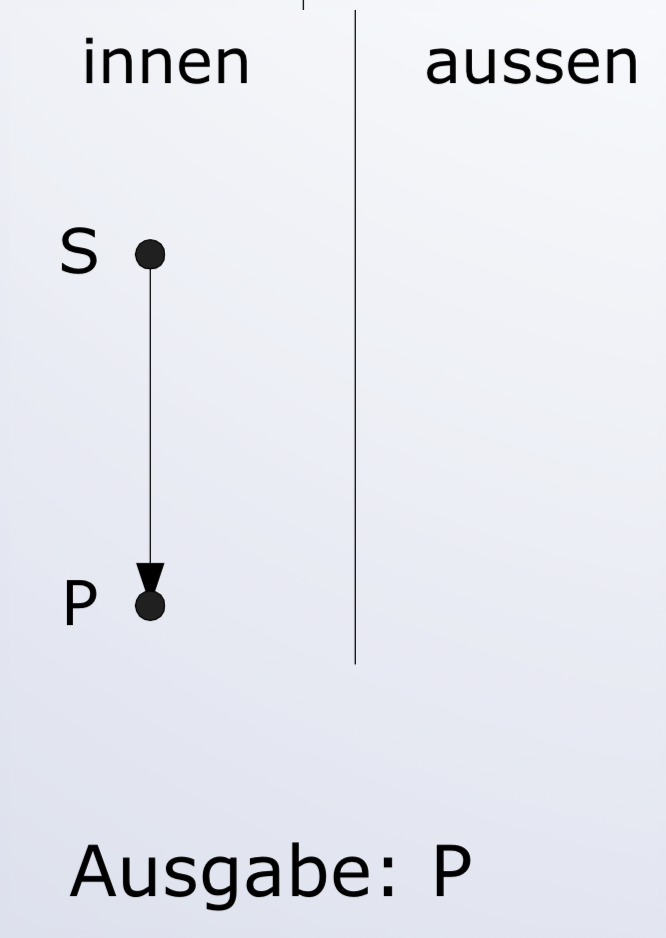
\includegraphics[width=0.2\textwidth]{assets/Sutherland-Hodgeman1.png}
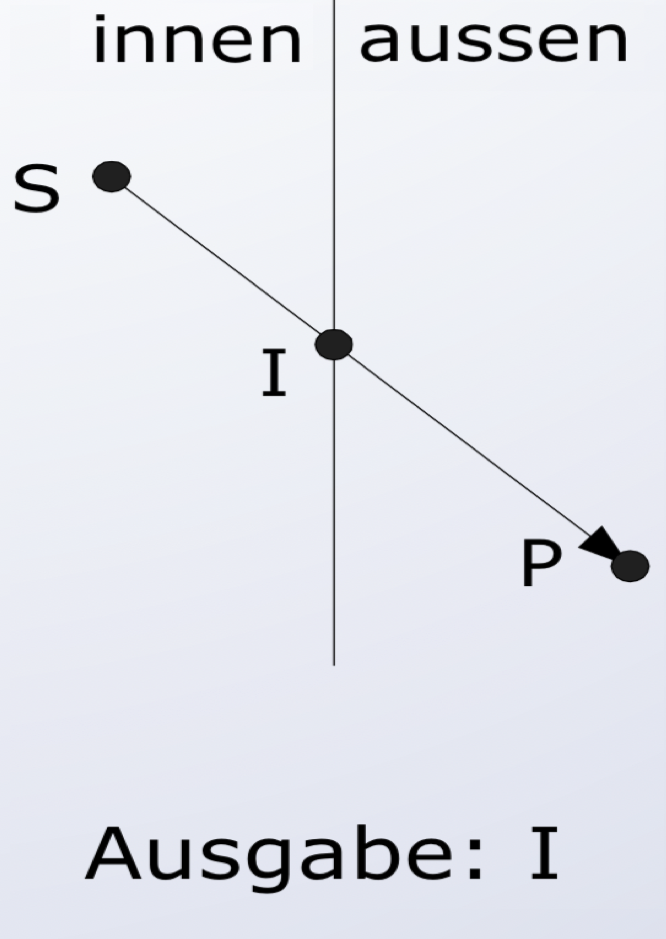
\includegraphics[width=0.2\textwidth]{assets/Sutherland-Hodgeman2.png}

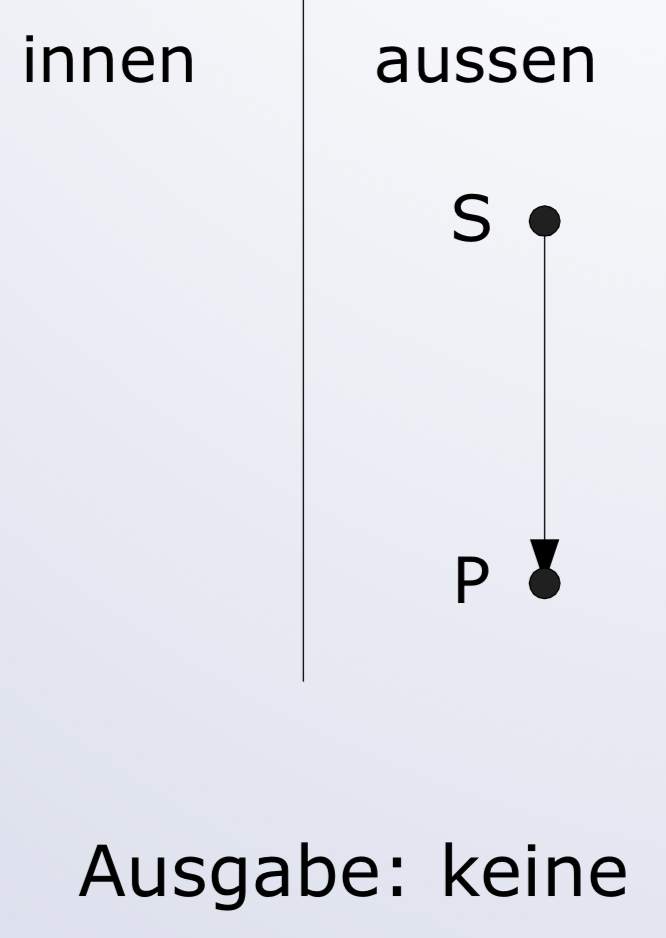
\includegraphics[width=0.2\textwidth]{assets/Sutherland-Hodgeman3.png}
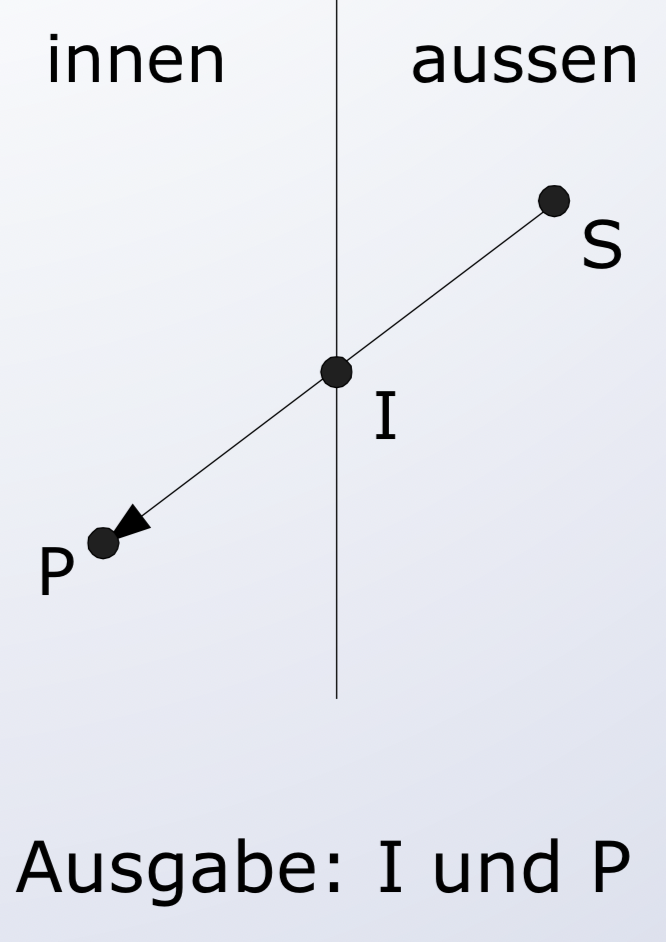
\includegraphics[width=0.2\textwidth]{assets/Sutherland-Hodgeman4.png}

\textit{Vorgehensweise: Verbindung zwischen zwei Punkten wird gemäss Regeln untersucht. 0-2 Eckpunkte des "neuen" Polygon als Ausgabe}

\textit{Beispiel nur an einer Kante:}

\begin{tabular}{cl}
    \begin{lstlisting}
Polygon 1:
ABCDE
  AB -> B
   BC -> B'
    CD -> -
     DE -> D'E
      EA -> A
Polygon 2:
BB'D'EA
\end{lstlisting} &
    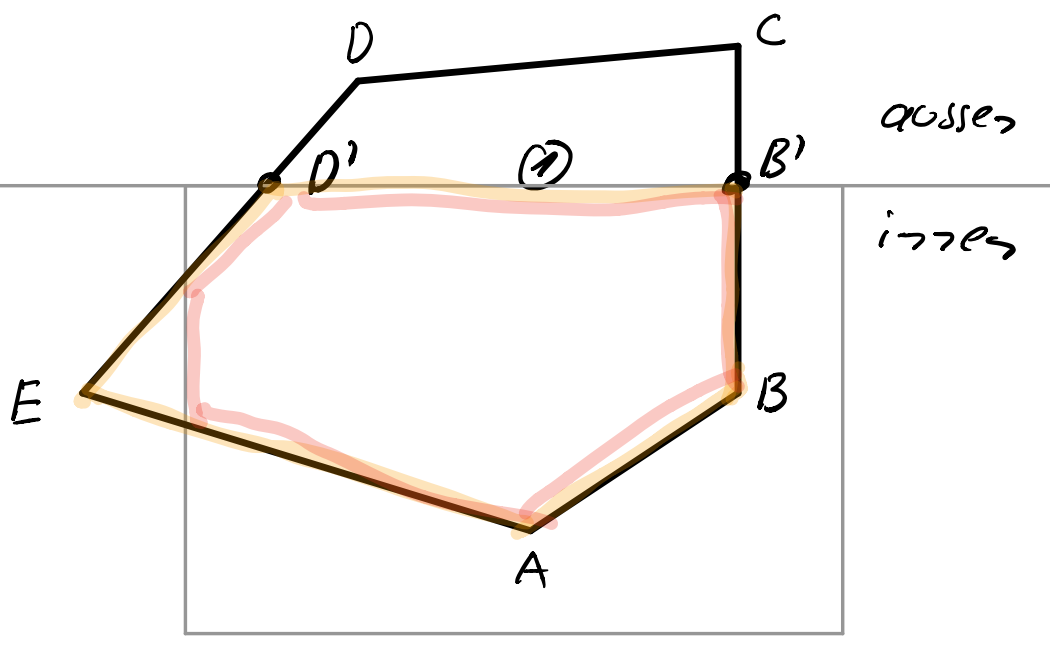
\includegraphics[width=0.25\textwidth]{assets/Sutherland-Hodgeman-example.png}
    \\

\end{tabular}
